% !TeX spellcheck = hu_HU
% !TeX encoding = UTF-8
% !TeX program = xelatex
%----------------------------------------------------------------------------
\section{A C4 futtatókörnyezet}\label{sec:c4:rt}
%----------------------------------------------------------------------------

Bár maga a C4 megvalósításom natív kódként fut (esetleg \gls{JIT} támogatással), vannak olyan megvalósítási kérdések, amelyeket a fordítóban nem lehetséges teljesen megvalósítani.
Ezekről szól ez az alfejezet.

\subsection{A dinamikus típusok kezelése}\label{subsec:c4:rt:types}

\Aref{sec:c4:desc}.~fejezet leírása alapján a C4 nyelv dinamikusan típusos.
Ez azt jelenti, hogy fordítási időben nem ismertek a tényleges típusai a használt objektumoknak, hanem futás közben derül ki, hogy mi van egy változóban.
A direkt módon futtatható ,,szkript'' nyelvek többségének ez a típusozása, mert így a kód írása közben elég fejben tartani, hogy mi és milyen típusú, nem kell kiírni minden hova, hogy egy változó {\tt int} típusú.
Ilyenre példa a Perl, Tcl, Ruby és Python nyelvek.

A dinamikusan típusos nyelvek közös megvalósítási elemei, hogy rendelkeznek egy valamilyen statikusan típusos nyelven (\pl C) megadott olyan adatszerkezettel, amelyik a dinamikus típust kezeli a futtatókörnyezet számára.
Három verzióban kerül ez gyakran megvalósításra.
Az első kettővel kapcsolatban bemutatom a problémákat, majd részletesen tárgyalom a harmadik, általam is használt megvalósítást.

Első, hogy valamilyen általános típusra mutató mutatót használ a rendszer és objektum\-/orientált technikákkal kezeli a típusok között fellépő különbségeket.
Ilyen a CPython által használt {\tt PyObject} objektumokra, amikre mutatókat ad át futás közben a különböző futó függvények számára.

Ez a megoldás szép, de hatékonysági problémákba ütközhet, hiszen minden objektum eléréséhez a mutatót követni kell a memóriában, hogy a mutatott értéket fel lehessen használni, és a memória elérés jelentősen lassabb, mint a processzor regisztereiben dolgozni.
Emellett megvan az a hátránya, hogy minden objektumba csomagolva kerül tárolásra.
Komplexebb típusok esetében ez nem kifejezetten probléma, viszont olyan alapvető típusoknál, mint egy 32 bites egész szám vagy egy darab {\tt double} lebegő pontos szám, ez jelentős memóriatöbblettel járhat.
Ennek a konkrét mértéke megvalósítástól függ.

Második, hogy egy összegtípus formájában tárolja a megfelelő értéket, azzal együtt, hogy mi a valós típusa.
Ilyen Perl számára az {\tt SV} típus, míg a (modern) Tcl-nek ez a {\tt Tcl\_Obj}.

Az általános naiv megvalósítása egy összegtípusnak azonban memória pazarló.
Tegyük fel, hogy a tárolt adatot egy 64-bites szám bitjeibe belekódolt mezőben tároljuk és mellette egy 8 bites mezőben azt, hogy mi a típusa annak, amit tárolunk.
Utóbbit ha előjel mentes számként értelmezzük, akkor 255 darab különböző típust tudunk megkülönböztetni.
Ha ez kevésnek tűnik, akár még 32 bittel is valamennyire érvényes a példa, bár kevésbé drasztikus az eredmény.

A 8 bit választása példának azonban nem véletlenszerű.
Amellett, hogy jól szemlélteti az említeni kívánt problémát, a jelenlegi felhasználási helyzetben egy valós és használható érték.
Abból eredően, hogy a C4 nyelvben nem lehetséges külön típusokat bevezetni olyan módon, hogy azt a nyelv futtatókörnyezete számára változást okozzon, nincs szükség nagy méretű típusjelölő mezőre.
Mivel minden C4-ben létrehozott ,,típus'' valamilyen konstruktor függvény által visszaadott megfelelő interfésszel rendelkező blokk (gyakran closure), így ezek mind egy típusnak látszanak a bitek szintjén: egy meghívható blokk.
Emiatt összesen -- az alább leírt optimalizációkkal együtt -- 4 különböző értékre van szükség a típus elkódolásához, amihez igazából 2 bitre van csak szükség, de a byte\footnote{Egy byte-ról a példa kedvéért felteszem, hogy 8 bit.} alapú címzés miatt és az esetleges bővíthetőség lehetősége miatt, a példa 8 bitet használ.

Az eddig felvezetett probléma pedig a következő: a 64-bites szám mérete 8 byte, és az igazítása (alignment) is általában 8 byte.
A 8-bites szám 1 byte, és az igazítása is 1 byte.
Ezeket az igazítási feltételeket érdemes figyelembe venni, különben vagy jóval lassabb lesz az olvasás az adott memória címről, vagy szimplán nem is megengedett (a konkrét processzor architektúrájától függően).
Így viszont, ha ezekből képzünk valami struktúra jellegű objektumot, akkor a 8 byte-os igazítás miatt kitöltő (padding) byte-okra van szükség, különben a 64-bites szám nem tudna 8 byte-os határon kezdődni.
Emiatt a teljes struktúra 128 bit memóriát foglal a ténylegesen használt 72 bit helyett, azaz a teljes memória majdnem felét elpazarolja.
Máshogy megfogalmazva, kicsivel kevesebb, mint kétszer annyi memóriát foglal minden ilyen formájú naiv összegtípus, mint amire ténylegesen szüksége van.
Ezt a helyzetet szemlélteti \aref{fig:bad-mem}.~ábra.
Nyilván még rosszabb eredményt kapunk, ha csak 2 bit értékes adattal számolunk, de ez már nem változtat lényegesen a hatékonyság fokán, és véleményem szerint, átlag számítógépek esetén byte méretű memória alá menni ilyen fajta optimalizációkkal nem kifizetődő.

\begin{figure}[htb]
    \centerline{
\includegraphics[width=.7\linewidth]{figures/bad-memory.pdf}}
    \caption{A naiv összegtípus memóriakihasználtságának ábrázolása}\label{fig:bad-mem}
\end{figure}

A harmadik lehetőség pedig a szükséges extra adat bedobozolása egy-egy adattípus által szabadon hagyott bitekbe.
Az extra adat lehet például az összegtípus aktív típust jelző adata, ami alapján a többi bit értékét lehet megfelelően értelmezni.

Két elterjedtebb technika van, amelyik ezt a koncepciót használja: a \gls{NaN} dobozolás (\gls{NaN} boxing) és mutató címkézés (pointer-tagging).
A \gls{NaN} dobozolás a technikát használja a SpiderMonkey JavaScript motor a Firefox böngésző alatt, a mutató címkézést pedig a V8 JavaScript motor a Chrome/Chromium böngészők és NodeJS platform alatt.

A \gls{NaN} dobozolás egy IEEE 754 \cite{noauthor_ieee_2019} \gls{NaN} értékének kihasználatlan bitjeit, míg a mutató-címkézés a mutató igazításából eredő alsó biteket használja erre a célra.
A \gls{NaN} dobozolásban az előjel bit és a mantissza mértéke válik felhasználhatóvá, ami összesen egy 64-bites {\tt double} érték esetén 53 bitnyi szabad tárhely; ebből le kell foglalni valamennyit a típus tárolására.
Ezzel szemben mutató címkézésnél alapból tipikusan az alsó 3 bit használható fel szabadon egy 64-bites architektúránál, mert a mutatók igazítása 8, ez azonban felülírható megfelelő módon foglalt memória használatával, így ez az érték módosítható.

A \gls{NaN} dobozolásnak előnye, hogy {\tt double} értékeket is tud egy az egyben tárolni extra memóriaigény nélkül.
Hátránya, hogy olyan processzorokon, amelyiken 5-szintű lapozás (5-level paging) van használatban \cite{intel_corporation_5-level_2017} nem egyszerűen használható, mert a szabadon maradt bitekben nem lehetséges eltárolni egy mutatót.
Utóbbi csak pár szerver és munkaállomás kategóriájú X86-64 (Intel és AMD \cite[8.2.~szekció]{advanced_micro_devices_inc_high_2023} is rendelkezik megvalósítással) processzorra terjed ki és ráadásul explicit módon be kell kapcsolni ezen a rendszereken is, hogy hatályban legyen.
Ezért nem találom egy nagy hátránynak a jelenlegi elvárások szerint, míg asztali számítógépek környezetében hatékonyság szempontjából egy hasznosabb tulajdonsága {\tt double} értékek natív kezelése indirekciót elkerülő módon.

Ezek alapján a C4 futtatókörnyezetének megvalósításához a \gls{NaN} dobozolás technikát valósítottam meg.
Ennek a technikának a C4 nyelv megvalósításában használt verzióját mutatom be a következő alszekcióban.

\subsubsection{A \gls{NaN} dobozolás technikája}\label{ssubsec:c4:rt:types:nan}

A \gls{NaN} dobozolás technikának alapvető kérdése, hogy milyen módon kerülnek a bitek kiosztásra.
Ennek elemi része, hogy milyen típusokat milyen módon érdemes támogatni.
Elsőként a négy alaptípus C4-ben, amit mindenképpen kezelni kell azok a következők: előjeles egész szám, 64-bites lebegőpontos szám, szöveg és végül blokk.
Utóbbi lehet függvény vagy closure, itt nem különböztetem meg őket, mert az egyszerű függvények implementálása megvalósítható a nulla hosszúságú kontextussal rendelkező függvényként.

Összesen a típusoknak 4 bitet használok fel: ez biztosít elég sok jövőbeli változást, illetve ezzel együtt 48 bit marad vissza az adatok tárolására, amelyik egy 8 többszörös, így a többi értékkel való munkát megkönnyíti.
Ezeket a típust tároló biteket a mantissza első 4 bitjén egyszerűen el lehet tárolni.

\begin{figure}[htb]
    \centerline{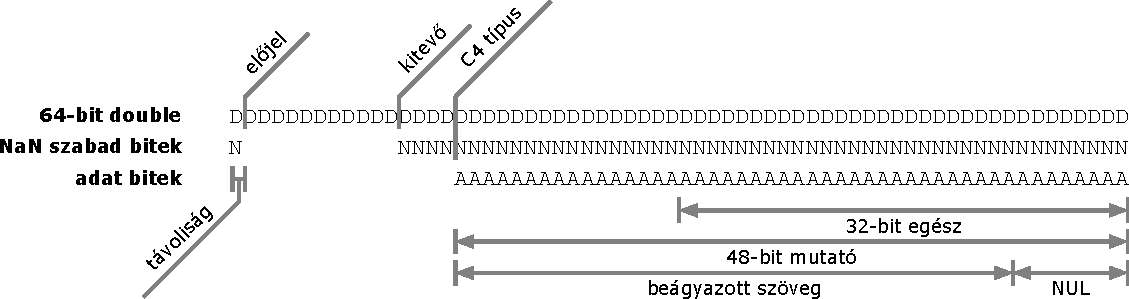
\includegraphics[width=\linewidth]{figures/bits.pdf}}
    \caption{A C4 által használt 64-bites {\tt double} bitjeinek kiosztása}\label{fig:bits}
\end{figure}

A \gls{NaN} értékben ki nem használt bitek közül van egy különálló bit, ami az eredeti lebegőpontos számban az előjelbitként viselkedik.
A \gls{NaN} értékben erre sincs szükség, így ezt az \un távoliság bitnek (remoteness bit) használom.
Ennek a feladata, hogy az adott típussal együtt lehetővé tegye eldönteni, hogy milyen módon van eltárolva az adat, ami az adott bitsorozathoz tartozik.
A távoliság bit beállításakor a lokálisan található bitek mindig egy mutatót tartalmaznak amelyik az adat típustól függő megvalósításra mutat, ellenkező esetben pedig valamilyen módon a lokális 64-bitben van elkódolva az adat.

A következő bekezdésekben leírom, hogy melyik típusú adat, milyen módon kerül eltárolásra a C4 futtatókörnyezetben.
Ezeket a paragrafusokat összefoglalja \aref{fig:bits}.~ábra a különböző módon használt bitek megjelölésével.

\paragraph{Lebegőpontos számok} Ezek a számok a \gls{NaN} dobozolás alaptulajdonságából eredően a legtöbb esetben automatikusan eltárolásra kerülnek, nem kell velük külön foglalkozni.
Egy sarkalatos eset van: egy tényleges \gls{NaN} érték, amelyik nem tartalmaz C4 által belekódolt információt.
Ezzel az egy esetnek van egy külön típuskód a lebegőpontos szám részére.
Ilyenkor az egész szám maga a valós adat.
Ezekből következően a távoliság bit sem kerül használatra.

\paragraph{Egész számok} Mivel a 32-bites számok sokszor elegendőek egy-egy érték tárolására, így az alsó 32 bit ki van jelölve ezeknek a tárolására, ha a típus egész számot jelöl.
Ilyenkor a távoliság bit nulla.
Abban az esetben, amikor a tárolandó számérték túllépi a 32-bites előjeles egész méretét, foglalásra kerül egy 64-bites szám tárhelye, és erre a számra mutató mutatót tárol az alsó 48 bit.

\paragraph{Szöveg} A szövegek legtöbb esetben hosszú karakterek sorozata, így ha a távoliság bit egy egy szöveget tároló adat esetén, akkor az alsó 48 bit egy mutató a karakterlánc elejére.
Ez a karaktersorozat egy \glslink{ASCII} NUL értékkel záródik, hogy a C függvényekkel kompatibilis legyen, azonban az első karakter előtti 64 biten található egy szám, amelyik a karakterlánc hosszát tárolja.
Ez egy optimalizáció, hogy ne lineáris időben lehessen meghatározni egy szöveg hosszát.

Egy másik optimalizációs stratégia, amelyet például a C++ szabványos könyvtár megvalósítások is használnak, az úgy nevezett rövid szöveg optimalizáció (short string optimization).
Ebben az esetben az általában tárolt mutató és hossz helyére memóriában nem egy tényleges mutatót és számértéket írnak, hanem a szöveg karaktereit.
Ezzel lehetséges a kis méretű dinamikus karakterlánc foglalások többségét megspórolni, illetve az olvasásnál is egy mutató indirekciót lehet spórolni.

Rövid szöveg optimalizációt megvalósít a C4 futtatókörnyezet is.
Azok a szöveg típusú adatok, amelyikben a távoliság hamis egy maximum 5 karakteres szöveget tárolnak alsó 48 bitben.
A legalsó 8 bit ilyenkor mindig csupa nulla, hogy C sztring kezelő függvényekkel kompatibilitást megmaradjon, de rövidebb mint 5 karakter esetén az összes nem használt alsó bit nulla.
Ez látszik a ,,beágyazott szöveggel'' jelölt részen \aref{fig:bits}.~ábrán is.
Meg kell jegyezne, hogy a jelenlegi megvalósításban ez csak alvég (little endian) processzorokon működik, így csak ilyen rendszeresen történik meg az optimalizáció.

\paragraph{Blokk} A blokkok a szövegekkel haszonló módon a legtöbb esetben egy mutatót tárolnak egy speciális byte sorozatra, amelyik a dinamikusan meghívható függvények adatait tárolja.
Erről az adatszerkezetről rövidesen lesz szó.
Ilyenkor a távoliság bit egy.

Ezek mellet azonban rendelkezik a C4 pár ,,nevezetes'' blokk értékkel, amikkel az azonosság ellenőrzése hatékonyabbá változtatható, ha a többi értéktől elkülönülő, globálisan egyedi reprezentációval rendelkezik.
Ilyen az üres blokk, és az igaznak és a hamisnak megfelelő logikai értékek.
Ezek C4 kódban mind megadható blokk elemek, így speciális kódolásuk csupán optimalizációs célt szolgál.
Mivel a blokk értékek olyan állapotát, ahol a távoliság bit hamis az eddigiek alapján nem használtam fel, így ezt a szabad tárolási lehetőséget használom ki ezeknek az értékeknek a tárolására.
A blokk típusú adatok tehát hamis lokalitás bit esetén egy-egy konstans értéket tárolnak az alsó 48 bitjükben, amelyik célja, hogy az ekvivalencia ellenőrzését két 64-bites szám összehasonlítására lehessen redukálni.

A függvények tárolására egy külön adatszerkezet kerül felhasználásra.
Ez egy metaadatokkal kezdődő byte sorozata azoknak az argumentumoknak, amivel meg kell hívni a függvényt.
A metaadatok értelmezéséről szól \aref{fig:fn-bytes}.~ábra.
Az egész egy memóriafoglalással kerül lefoglalásra, és alapból nincsenek kitöltve az argumentumokra vonatkozó byte-ok értékei.
Ezeket lehetséges előre, részletekben beletölteni, vagy az adat függvényként hívásakor megadni; mind két esetben a meglévő memóriaterületre másolódnak, és az kerül megfelelő részekre bontással átadásra.
A kontextus, amennyiben létezik, is itt kerül eltárolásra, az argumentumok előtt; a mérete fel van kerekítve a következő 16 többszörösére, és csak méretének csak $\frac{1}{16}$-a kerül tárolásra.
Ez a művelet teszi lehetővé, hogy a 2 byte-on tárolt méret ellenére nagyobb méretű kontextusokat is képes legyen tárolni.
A nem használt mezőt régebbi verziók használták, és a jövőbeli verziók által használatra van fenntartva, értéke sosem definiált.

\begin{figure}[htb]
    \centerline{
\includegraphics[width=.6\linewidth]{figures/fn-mem.pdf}}
    \caption{A függvényeket tároló adatszerkezet}\label{fig:fn-bytes}
\end{figure}

\subsection{A lusta kiértékelés}\label{sec:c4:rt:pkg}

A lusta kiértékelés a másik fordítási időben nem általánosan megvalósítható tulajdonsága a C4 nyelvnek.
Minden függvényhívás esetén, az argumentumok nem kerülnek meghívásra, amíg a megfelelő paraméter értékét nem próbálja elérni a hívott függvény.
Emiatt az átlagos függvényhívási sablon -- amelyiket a hardver is támogat -- nem használható direkt módon, hiszen nem tud egy olyan ,,objektumként'' átadni paramétereket, amelyek híváskor futnak le, csak direkt kimeneteket.

Emiatt a C4 nyelvű függvények {\tt c4rt\_package\_t} típusú objektumként várják el minden paraméterüket.
Ez egy 16 byte-os adatstruktúra, aminek a byte-jainak értelmezése megtalálható \aref{fig:pkg-mem}.~ábrán.
Az ezen látható ,,adatok'' mező több különböző értéket tárolhat a struktúra jelenlegi állapotának függvényében, így ennek a tárgyalása következik a következő paragrafusban.
A különböző állapotoknak a megkülönböztetésére is szolgálnak a egyéb mezők a struktúrában, amelyek láthatóak az ábrán.
Az adat típushoz hasonlóan a nem használt mezőt itt is régebbi verziók használták, és fenn van tartva a jövőbeli verziók által való használatra.

\begin{figure}[htb]
    \centerline{
\includegraphics[width=.35\linewidth]{figures/package-mem.pdf}}
    \caption{A függvényeket tároló adatszerkezet}\label{fig:pkg-mem}
\end{figure}

Ebben négy elkülönülő állapotban lehetséges különböző adatokat olvasni:
Elsőként, az eredményt adó függvény még nem lett kiértékelve és annak aritása nulla.
Ilyenkor az ,,adatok'' mezőben egy függvénymutató található, amelyiket nulla argumentum átadásával meg lehetséges hívni és visszaad egy dinamikus típusú adat objektumot.
Amennyiben a függvénynek vannak paraméterei és/vagy kontextusa, akkor a függvénymutató helyett egy olyan struktúrára mutató mutató található, amelyiknek az elején a számítást végrehajtó függvény mutatója, majd utána a híváshoz szükséges összes adat: kontextus byte sorozata, ha van, majd a paraméterek, ha vannak.
Az utóbbi esetnek egy speciális esete, amikor egy adat objektumba csomagolt függvényt tárol, ilyenkor ez kerül bele az ,,adatok'' mezőbe.
Végül, ha a számítás már egyszer megtörtént, akkor az eredményként kapott adat található meg ezeken a byte-okon.

Külön figyelmet igényel, amikor a hívott függvény rendelkezik kontextussal (tehát a C4 nyelvbeli megfelelője egy closure volt).
Ilyenkor ezt is külön módon el kell tárolni és a függvény hívásakor azt megfelelő módon elérhetővé kell számára tenni.
Ezt az egyszerű adat objektumokban tárolt függvények kontextusainál használt megoldással analóg módon a méretének $\frac{1}{16}$-át tárolva és az egyéb tárolt adatok elejére másolásával valósítom meg.
